The scaled logit model was fit using the maximum likelihood method. The fitted protection curves are in Figure \ref{fig:fit-sclr-prot}.

\begin{figure}[htp]
	\centering
	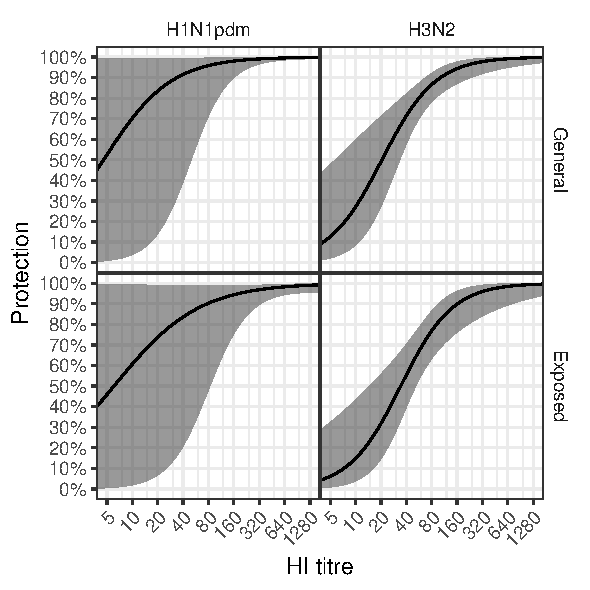
\includegraphics[width=0.8\textwidth]{../fit-sclr-plot/hanam-hi-prot.pdf}
	\caption{
	Fitted protection curves and confidence intervals from the scaled logit fit to Ha Nam data (also shown in Figure \ref{HanamCounts}) using the maximum likelihood method. The solid line is the point estimate. The shaded region is the 95\% confidence interval.
	}
	\label{fig:fit-sclr-prot}
\end{figure}

There is not enough data in the H1N1pdm subset to generate useful estimates. For H3N2 subset, limiting the sample to just those exposed to the virus (at least one household infection in a season) improved the precision of the estimates. The general lack of precision in the estimates is likely due to the number of parameters in the model (3 parameters with 1 covariate) and the censored nature of HI titre measurements, particularly the fact that any titre below 10 is undetectable which means that it is impossible to distinguish between many of the observations (e.g. some subjects with undetectable titres may have had a true titre of 9 while others --- of 2, but both were recorded as 5) which makes it harder to estimate the baseline probability (as seen in the confidence bounds increasing at small (<10) titres).
